\documentclass[11pt,twoside]{article}

\usepackage[utf8]{inputenc}
\usepackage{easyReview}
\usepackage{geometry}
\geometry{
	a4paper,
	left=40mm,
	right=20mm,
	top=20mm,
	bottom=20mm
}


% Fonts
\usepackage[T1]{fontenc}
\usepackage[scaled]{helvet}
\renewcommand*{\familydefault}{\sfdefault}

% Section heading font size
\usepackage{titlesec}
\titleformat{\section}{\normalfont\fontsize{14}{15}\bfseries}{\thesection}{1em}{}
\titleformat{\subsection}{\normalfont\fontsize{12}{15}\bfseries}{\thesubsection}{1em}{}
\titleformat{\subsubsection}{\normalfont\fontsize{11}{15}\bfseries}{\thesubsubsection}{1em}{}

% No indentation for new paragraphs
\setlength{\parindent}{0pt}

% Line spacing
\newcommand{\commonlinespread}{1.5}
\newcommand{\toclinespread}{1.0}
\linespread{\commonlinespread}

% Section heading spacing
\usepackage{titlesec}
\titlespacing\section{0pt}{12pt plus 2pt minus 2pt}{6pt plus 2pt minus 2pt}
\titlespacing\subsection{0pt}{12pt plus 2pt minus 2pt}{6pt plus 2pt minus 2pt}
\titlespacing\subsubsection{0pt}{12pt plus 2pt minus 2pt}{6pt plus 2pt minus 2pt}

% Header and footer
\newcommand{\changehdrfont}{%
	\fontsize{10}{11}\selectfont
}
\usepackage{fancyhdr}
\pagestyle{fancy}
\fancyhf{} % clear fields
\fancyhead[LE,RO]{\changehdrfont\leftmark}
%\fancyhead[LE,RO]{\changehdrfont\rightmark}
%\fancyhead[RE,LO]{\changehdrfont\thepage}
%\fancyhead[RE,LO]{\chaptername\space\thechapter}
%\fancyfoot[CE,CO]{Name}
\fancyfoot[LE,RO]{\thepage}

% TOC dots
\usepackage{tocloft}
\renewcommand{\cftpartleader}{\cftdotfill{\cftdotsep}} % for parts
\renewcommand{\cftsecleader}{\cftdotfill{\cftdotsep}} % for sections

% Redefine chapter to include a page break after
%\usepackage{letltxmacro}
%\LetLtxMacro{\oldchapter}{\chapter}
%\renewcommand{\chapter}[2][]{\oldchapter[#1]{#2}\vspace{\fill}\par\pagebreak}

\usepackage[ngerman,english]{babel}
%\usepackage{breakurl} % not required with pdflatex

\usepackage{graphicx}
%\usepackage{amsfonts}
\usepackage{amssymb}
\usepackage{amsmath, bm}
\usepackage{hyphenat}
\usepackage{siunitx} % spacing between value and its unit
\usepackage{gauss}
\usepackage{float}
\usepackage{pdflscape}
\usepackage{tabularx}
\usepackage{multirow}
\usepackage{setspace}
\usepackage{subcaption}
\usepackage{dcolumn}

\usepackage[format=hang,font=small,labelfont=bf]{caption}
\captionsetup{justification = raggedright, singlelinecheck = false, }

\usepackage{endnotes}
\let\fnote\footnote

%\usepackage{pdflscape}
\usepackage{epstopdf}
%\usepackage{subfig}
\usepackage{booktabs}
\usepackage[right]{eurosym}
%\usepackage{setspace}	% package used to make double space between lines
\usepackage{longtable}
\usepackage[flushleft]{threeparttable}
\usepackage{rotating}

\definecolor{darkblue}{rgb}{0.055,0.094,0.588}
\definecolor{darkred}{rgb}{0.4,0,0.0157}
\definecolor{myblue}{rgb}{0.2,0.2,0.7}
\definecolor{myred}{rgb}{0.9,0,0}
\newcommand{\jemph}[1]{{\color{myblue}#1}}
\newcommand{\remph}[1]{{\color{myred}#1}}

\newcommand{\commentbox}[1]{\fcolorbox{red}{yellow}{\begin{minipage}{\textwidth}
			\begin{footnotesize}#1\end{footnotesize}\end{minipage}}}

\usepackage{chngcntr}
\counterwithin*{equation}{section}
\counterwithin*{equation}{section}

\usepackage[affil-it]{authblk}

\usepackage{hyperref}
\newcommand{\samecolor}{0,0,.8}
\hypersetup{
	colorlinks = true,     % Colours links instead of ugly boxes
	urlcolor   = darkblue, % Colour for external hyperlinks
	linkcolor  = darkblue, % Colour of internal links
	citecolor  = darkblue  % Colour of citations
}

\usepackage[nameinlink,capitalize]{cleveref}

\newcommand\PlaceInsert[1]{
	\begin{center}
		\framebox{Insert \Cref{#1} here.}
	\end{center}
	\bigskip}


\newlength{\drop}

\usepackage{subfiles}
\usepackage[]{blindtext}
\usepackage{csquotes}

\usepackage[style=apa,backend=biber,natbib=true,uniquename=false,pagetracker=true]{biblatex}
\addbibresource{paper.bib}
\DeclareSourcemap{ %suppress printing url and doi in bibliography
	\maps{
		\map{
			\step[fieldsource=url,
			match=\regexp{.*},
			fieldset=url, null]
			\step[fieldsource=doi,
			match=\regexp{.*},
			fieldset=doi, null]
		}
	}
}

\newcommand{\titelderarbeit}{Hier den Titel der Arbeit einfügen}

\begin{document}

\selectlanguage{ngerman}
\pagenumbering{roman}

\begin{titlepage}
	\begin{tikzpicture}[remember picture,overlay]
		\node[anchor=north east,yshift=-1.25cm,xshift=-1.5cm]
		at (current page.north east)
		{
\includegraphics[width=0.25\textwidth]{./onlineplus}};
	\end{tikzpicture}

	\vspace{4cm}
	\centering
	Hochschule Fresenius\\
	Fachbereich onlineplus\\

	Studiengang: Studiengang\\

	\vspace*{3cm}
	Art der Arbeit (Hausarbeit, \ldots)
	\vspace*{1cm}

	{\textbf{\huge{\titelderarbeit}}}

	\vspace*{2cm}

	Vorname Name \\
	Matrikelnummer: xxx\\

	\vspace*{1cm}
	Modul: xxx\\
	Dozent: xxx\\
	Abgabedatum: xxx

	\vspace*{.5cm}
\end{titlepage}

\clearpage

\linespread{\toclinespread}

\tableofcontents{}
\clearpage
\listoffigures
\clearpage
\listoftables
\clearpage

\linespread{\commonlinespread}

\pagenumbering{arabic}

\section{Einleitung}\label{sec:einleitung}

\citet[1]{lebowski1998} \blindtext % Ein Zitat und Text

\section{Kapitel}\label{sec:kapitel}
\blindtext

\subsection{Unterkapitel A}\label{subsec:unterkapitel-a}
Beispiel für eine Abbildung: \\
\begin{figure}[H]
	\caption{Studierende nach Bundesland}
	\label{fig:studis}
	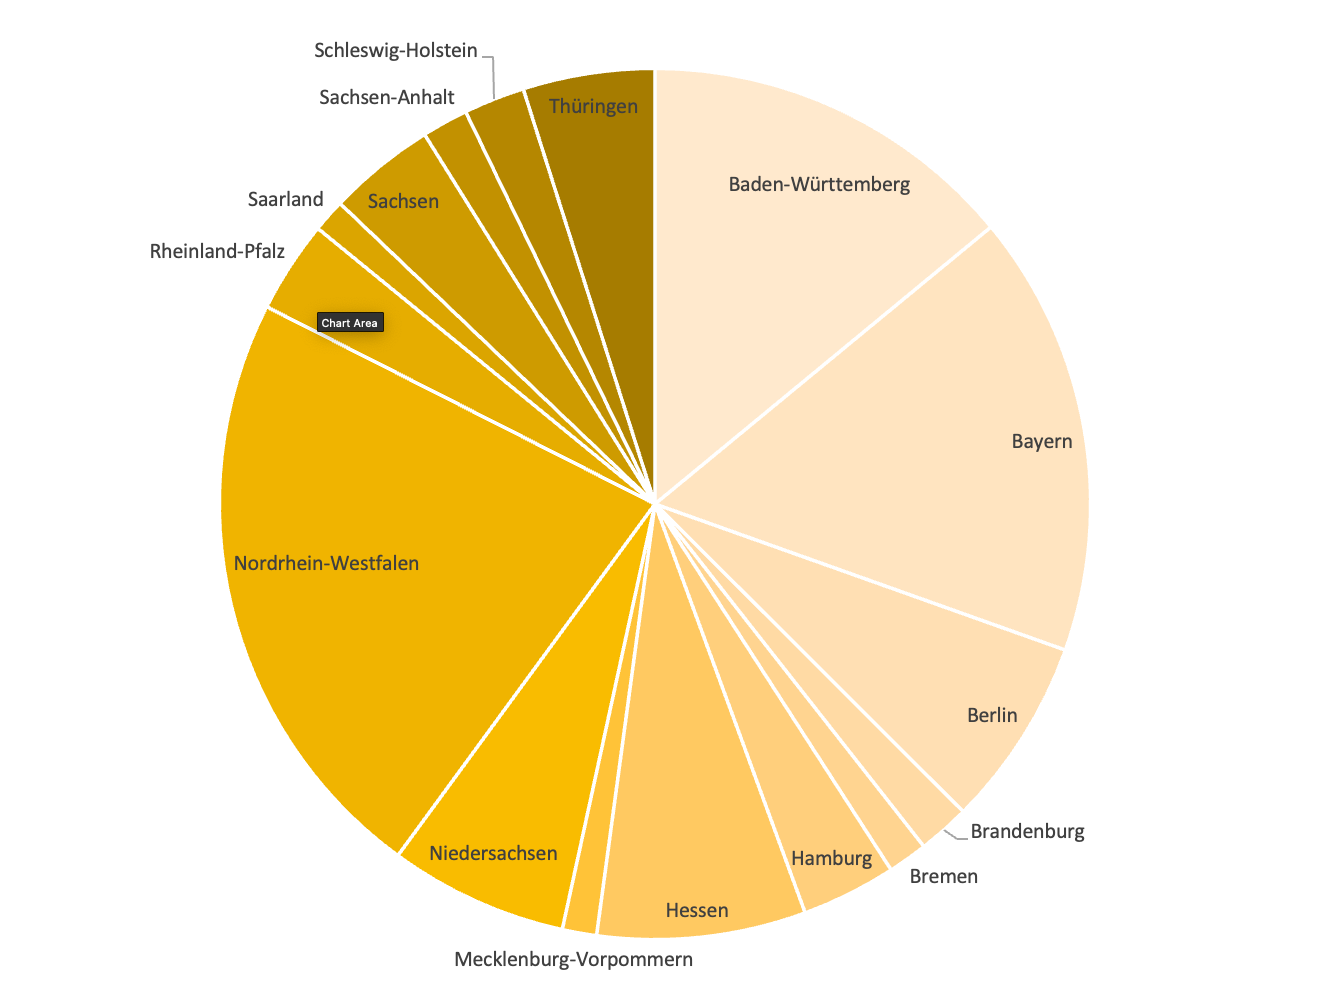
\includegraphics[width=6cm]{studierende_nach_bundesland}
	\footnotesize
	Quelle: eigene Darstellung in Anlehnung an Statistisches Bundesamt, 2023
\end{figure}

\subsection{Unterkapitel B}\label{subsec:unterkapitel-b}

Beispiel für eine Tabelle: \\

\begin{table}[H]
	\caption{Studierende nach Bundesland und Geschlecht}
	\begin{tabular}{|l|r|r|r|}
		\toprule
		\textbf{Bundesland}    & \textbf{männlich} & \textbf{weiblich} & \textbf{Insgesamt} \\
		\midrule
		Baden-Württemberg      & 27830             & 28030             & 55860              \\
		Bayern                 & 32917             & 32462             & 65379              \\
		Berlin                 & 13056             & 14964             & 28020              \\
		Brandenburg            & 3813              & 3864              & 7677               \\
		Bremen                 & 2846              & 3014              & 5860               \\
		Hamburg                & 6498              & 7511              & 14009              \\
		Hessen                 & 14560             & 16291             & 30851              \\
		Mecklenburg-Vorpommern & 2199              & 2871              & 5070               \\
		Niedersachsen          & 12304             & 14116             & 26420              \\
		Nordrhein-Westfalen    & 43088             & 46238             & 89326              \\
		Rheinland-Pfalz        & 6185              & 7459              & 13644              \\
		Saarland               & 2426              & 2440              & 4866               \\
		Sachsen                & 7666              & 8257              & 15923              \\
		Sachsen-Anhalt         & 3261              & 3577              & 6838               \\
		Schleswig-Holstein     & 4594              & 4422              & 9016               \\
		Thüringen              & 7542              & 11943             & 19485              \\
		\bottomrule
	\end{tabular}
	\footnotesize \\\\ Quelle: eigene Darstellung in Anlehnung an Statistisches Bundesamt, 2023
	\label{tab:studis}
\end{table}

\clearpage
\printbibliography[heading=bibintoc]

\clearpage
\textbf{Eidesstattliche Erklärung}\\

Hiermit versichere ich, dass ich die vorliegende Arbeit mit dem Titel ``\titelderarbeit''
selbstständig und ohne fremde Hilfe verfasst und keine anderen als die angegebenen Hilfsmittel
verwendet habe.\\

Die Stellen der Arbeit, einschließlich Tabellen und Abbildungen, die anderen Werken dem Wortlaut
oder dem Sinn nach entnommen sind, habe ich in jedem einzelnen Fall kenntlich gemacht und die
Herkunft nachgewiesen.\\

Die Arbeit hat in gleicher oder ähnlicher Form noch keiner anderen Prüfungsbehörde vorgelegen und
wurde noch nicht veröffentlicht.\\


\vspace{1.5cm}
\begin{tabular}{@{}p{4cm}p{1cm}p{8cm}@{}}
	\hrulefill &  & \hrulefill                \\
	Ort/Datum  &  & Eigenhändige Unterschrift \\
\end{tabular}

\end{document}